% intro %

As its name suggests, high energy physics research is performed by studying subatomic particle collisions at very high energies. (fix me).
<<<<<<< HEAD
This section provides details about the Large Hadron Collider (LHC), and proton's journey toward the LHC. %and description of the CMS detector.  (fix me) 

%\subsection{The large hadron collide}
The LHC is the most powerful particle accelerator in the world in the present time. 
The LHC ring is quite large, about 27 km in circumference, and it collides Hadrons, such as protons or heavy ions, by accelerating then in opposite dierections and colliding them at four points around LHC ring. 
%by traveling into two beams in opposite directions, and colliding at four points around LHC ring.

The LHC is a part of the CERN accelerator complex and sits in a tunnel 100 meters underground at CERN, the European Organization for Nuclear Research, on the border of Switzerland and France near Geneva, as shown in Fig.~\ref{fig:LHC_location}. The CERN accelerator complex consists of a succession of machines where each machine accelerates a beam of particles to a given energy before injecting the beam into the next machine in the chain. LHC is the last element of this chain where it is designed to collide particles at the ceneter-of-mass energy up to 14 TeV as shown in the figure Fig.~\ref{fig:acceleration_complex}

%The LHC is made of eight arcs and eight insertions. The arcs contain the dipole ,bending, magnets. The layout of the straight section depends on the specific use of the insertion: physics (beam collisions within an experiment), injection, beam dumping or beam cleaning.

%At the LHC we have 9 experiments: ALICE, %study heavy ion collisions, QGP,
%ATLAS, CMS %(general purpose detectors),
%LHCb %(study matter – antimatter asymmetry),
%LHCf %(shares intersection with ATLAS), 
%TOTEM %(shares intersection with CMS),
%MoEDAL-MAPP %(shares intersection with LHCb),
%FASER,
%SND@LHC. %(maybe add table with each experiment name and purpose/llocation)

\subsection{The journey of protons to the LHC}
It all starts from: a compressed tank of hydrogen that is connected to source chamber of the linear accelerator. The Linear accelerator 4 (Linac4) is designed to boost negative hydrogen ions (H with extra electron) to high energies that is corresponsing to to 1/3 of the speed of light (c) for the proton. Then the particles are fed to the booster stage this is Proton Synchrotron Booster (PSB).

At the PSB injection point a stripping foil will strip the electrons off the hydrogen anions creating protons that are accumulated as beam bunches in the four PSB rings. These proton bunches are then recombined at the exit of the PSB and further transferred down the CERN injector chain which accelerates the protons up to 91.6\% of $C$. After that the beam is sent to the Proton Synchrotron (PS) where the increase of energy does not transfer to velocity. Instead, it will increase the relativistic mass accelerating protons up to 99.9\% of $C$. Then the protons go to the super proton synchrotron (SPS).
=======
This section provides details about the Large Hadron Collider (LHC), and the proton's journey toward the LHC. %and description of the CMS detector.  (fix me)

%\subsection{The large hadron collide}
The LHC is the most powerful particle accelerator in the world in the present time.
%KenH From its name it is the LHC ring is quite large,
The LHC ring is quite large, about 27 km in circumference, and it collides hadrons, such as protons or heavy ions,
by accelerating them in opposite directions and colliding them at four points around the LHC ring.

The LHC is a part of the CERN accelerator complex and sits in a tunnel 100 meters underground at CERN, the European Organization for Nuclear Research, on the border of Switzerland and France near Geneva, as shown in Fig.~\ref{fig:LHC_location}. The CERN accelerator complex is a succession of machines where each machine accelerates a beam of particles to a given energy before injecting the beam into the next machine in the chain. LHC is the last element of this chain where it is designed to collide particles at the center-of-mass energy up to 14 TeV as shown in Fig.~\ref{fig:acceleration_complex}

%The LHC is made of eight arcs and eight insertions. The arcs contain the dipole ,bending, magnets. The layout of the straight section depends on the specific use of the insertion: physics (beam collisions within an experiment), injection, beam dumping or beam cleaning.
%% At the LHC we have 9 experiments:
%% ALICE (study heavy ion collisions, QGP,
%% ATLAS, CMS (general purpose detectors),
%% LHCb (study matter – antimatter asymmetry),
%% LHCf (shares intersection with ATLAS),
%% TOTEM (shares intersection with CMS),
%% MoEDAL-MAPP (shares intersection with LHCb),
%% FASER,
%% SND@LHC. (maybe add table with each experiment name and purpose/llocation)
The LHC hosts nine major experiments, each with distinct scientific objectives:
\begin{itemize}
\item {\bf ALICE} – Investigates heavy-ion collisions and quark-gluon plasma (QGP).
\item {\bf ATLAS \& CMS} – Multi-purpose detectors exploring a wide range of physics, including the Higgs boson and new particles.
\item {\bf LHCb} – Focuses on matter-antimatter asymmetry and heavy flavor physics.
\item {\bf LHCf} – Studies forward physics and cosmic ray interactions, sharing an intersection with ATLAS.
\item {\bf TOTEM} – Examines proton-proton scattering, sharing an intersection with CMS.
\item {\bf MoEDAL-MAPP} – Searches for highly ionizing particles and physics beyond the Standard Model, located near LHCb.
\item {\bf FASER} – Detects long-lived particles and neutrinos from LHC collisions.
\item {\bf SND@LHC} – Dedicated to studying neutrinos produced at the LHC.
\end{itemize}

\subsection{The journey of protons to the LHC}
%KenHH It all starts from: a compressed tank of hydrogen that is connected to source chamber of the linear accelerator. The Linear accelerator 4 (Linac4) is designed to boost negative hydrogen ions (H with extra electron) to high energies that is corresponsing to to 1/3 of the speed of light (c) for the proton. Then the particles are fed to the booster stage this is Proton Synchrotron Booster (PSB).
The process of producing a beam of protons begins with a compressed hydrogen tank supplying gas to the source chamber of Linear Accelerator 4 (Linac4). Linac4 accelerates negative hydrogen ions (H$^{-1}$), consisting of a proton with an extra electron, to high energies.
These ions reach speeds of approximately one-third the speed of light ($c$) before being stripped of their electrons. The resulting protons are then injected into the Proton Synchrotron Booster (PSB), where they undergo further acceleration.

At the Proton Synchrotron Booster (PSB) injection point, a stripping foil removes the electrons from the negative hydrogen ions, converting them into protons. These protons are then accumulated and organized into beam bunches within the four PSB rings for subsequent acceleration.
%At the PSB injection point a stripping foil will strip the electrons off the hydrogen anions creating protons that are accumulated as beam bunches in the four PSB rings.
These proton bunches are then recombined at the exit of the PSB and further transferred down the CERN injector chain which accelerates the protons up to 91.6\% of $c$.
After that the beam is sent to Proton Synchrotron (PS) where the increase of energy does not transfer to velocity.
Instead, it will increase the relativistic mass accelerating protons up to 99.9\% of $c$. Then the protons are sent to the Super Proton Synchrotron (SPS).
>>>>>>> origin/dev

%KenH Finally, at the LHC has two vacuum pipes where the protons will be going into different directions.
Finally, the LHC features two vacuum pipes, each carrying protons traveling in opposite directions.
The 27 km ring of superconducting magnets keep protons in the ring,
while accelerating structures called radio frequency (RF) cavities boost their energy.
%also the accelerating structures known as radio frequency (FR) cavities boost the energy.
%The LHC’s RF cavities bring the 450 GeV energy of the particles (1 GeV = 1 billion electron volts) to 6.5 TeV source.
The LHC's RF cavities increase the protons' energy from 450 GeV to 6.5 TeV (1 GeV = 1 billion electron volts).
The maximum energy is reached in around 20 minutes with the bunches having passed through the RF cavities more than 10 million times.
%There are four  points where the protons are collided, and CMS is one of the them which is the focus in thesis is focus on.
There are four locations along the ring where the protons are made to collide.
The CMS experiment is located at one of four collision points, which is the primary focus of this thesis.

 %------------ figures ------------%
\begin{figure}[t!]
\centering
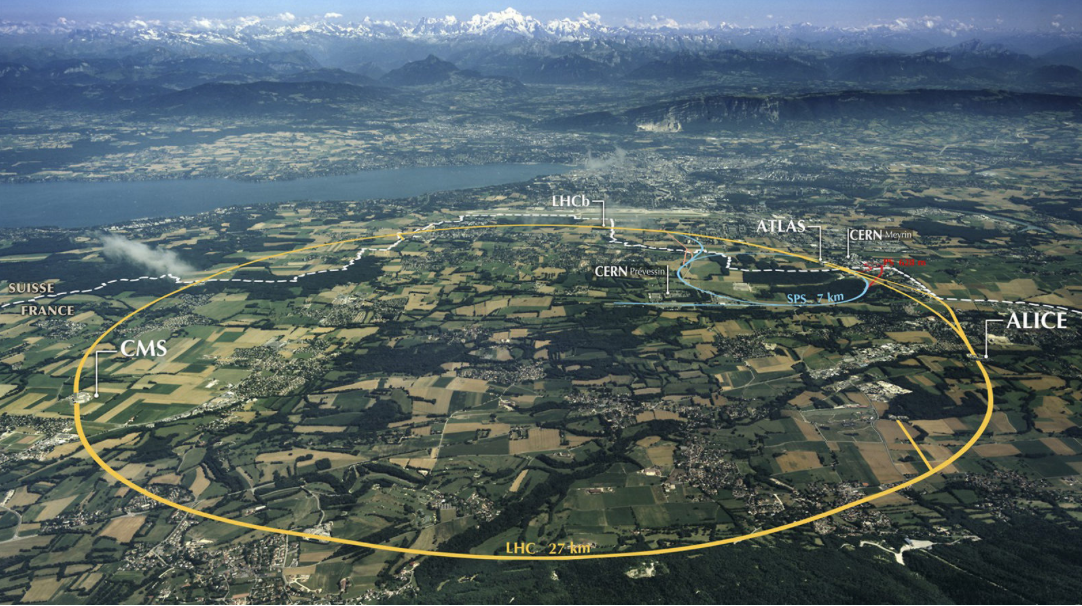
\includegraphics[width=0.99\textwidth]{figures/LHC_location.png}
<<<<<<< HEAD
\caption{The Location of the LHC}.Figure source~\cite{SMtable}.
=======
\caption[An aerial view of the LHC near Geneva, Switzerland]{An aerial view of the LHC near Geneva, Switzerland. Figure source~\cite{SMtable}.}
>>>>>>> origin/dev
\label{fig:LHC_location}
\end{figure}

\begin{figure}[t!]
\centering
<<<<<<< HEAD
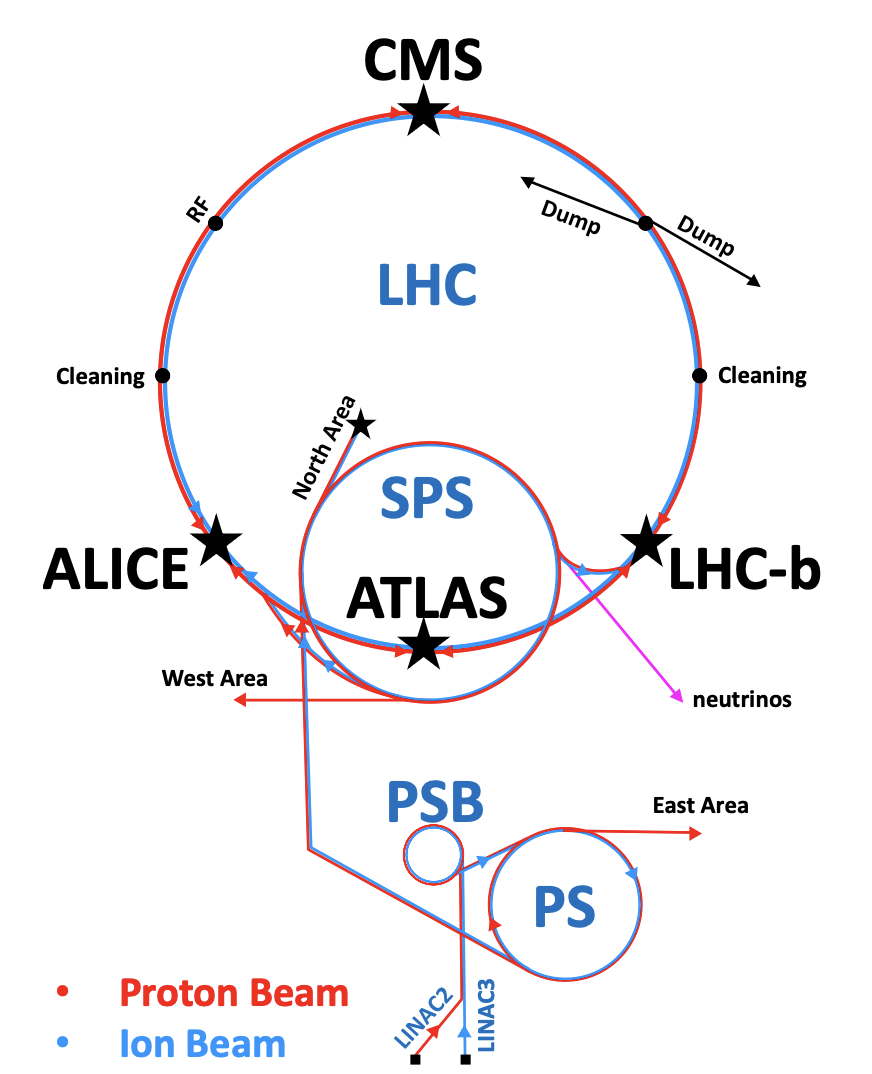
\includegraphics[width=0.50\textwidth]{figures/acceleration_chain.png}
\caption{Acceleration Complex}. Figure source~\cite{SMtable}.
=======
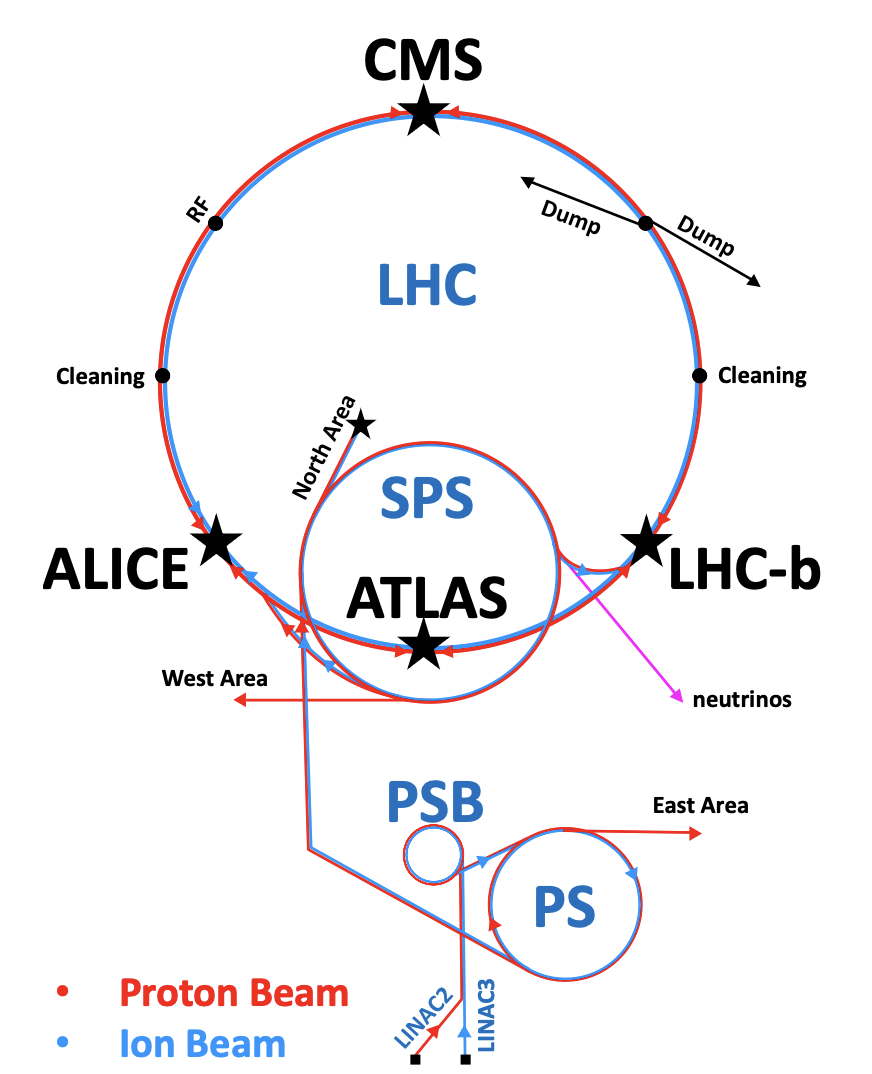
\includegraphics[width=0.99\textwidth]{figures/acceleration_chain.png}
\caption[CERN accelerator complex]{Overview of the CERN accelerator complex. Figure source~\cite{SMtable}.}
>>>>>>> origin/dev
\label{fig:acceleration_complex}
\end{figure}
